\documentclass{standalone}
\usepackage{PhysicalChemistryNote}
\begin{document}
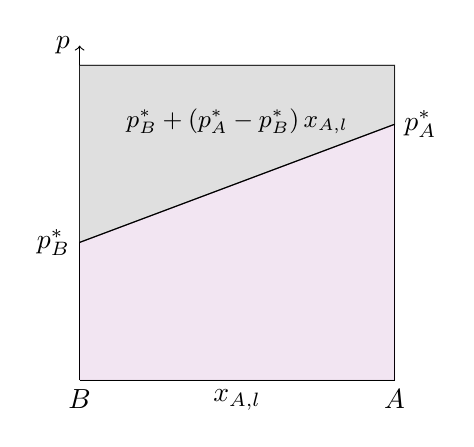
\begin{tikzpicture}
    \draw[-] (0,0) -- (4,0);
    \draw[->] (0,0) -- (0,4.25) node[left]{$p$};
    \draw[-] (4,0) -- (4,4);
    \draw[-] (0,4) -- (4,4);
    \node[below] at (0,0) {$B$};
    \node[below] at (4,0) {$A$};
    \node[below] at (2,0) {$x_{A,\l}$};
    \filldraw[fill=lightgray,opacity=0.5] (0,1.75) -- (4,3.25) -- (4,4) -- (0,4);
    \filldraw[fill=violet,opacity=0.1] (0,1.75) -- (4,3.25) -- (4,0) -- (0,0);
    \node[left] at (0,1.75) {$p_B^\ast$};
    \node[right] at (4,3.25) {$p_A^\ast$};
    \node[above] at (2,3) {\small{$p_B^\ast+\left(p_A^\ast-p_B^\ast\right)x_{A,\l}$}};
    \draw[-] (0,1.75) -- (4,3.25);
    
\end{tikzpicture}
\end{document}